
% np.sqrt()
% np.round( , num_decimals)
% np query syntax
% np.append
% np.flip
% two kinds of sorting
% remove (by index  and by value?)

% indexing, slices

\chapter{\huge Associative arrays in Python (2 of 2)}
\label{ch:arraysInPython2}

\index{series@\texttt{Series} (Pandas)}
K, now we can create \texttt{Series}es; let's figure out what we can do with
them.

\section{Accessing individual elements}

\index{element}
\index{len@\texttt{len()}}

We can use the same \texttt{len()} function in yet a third way: to ascertain
the number of key/value pairs in a series. Using the Figure~\ref{fig:Series}
example (p.~\pageref{fig:Series}):

\begin{Verbatim}[fontsize=\small,samepage=true,frame=single,framesep=3mm]
print(len(alter_egos))
\end{Verbatim}

\begin{Verbatim}[fontsize=\small,samepage=true,frame=leftline,framesep=5mm,framerule=1mm]
4
\end{Verbatim}

\index{boxies (square brackets)}
\index{[]@\texttt{[]} (boxies)}

Accessing the value for a given key uses exactly the same syntax that NumPy
arrays used (boxies), except with the key in place of the numeric index:

\begin{Verbatim}[fontsize=\small,samepage=true,frame=single,framesep=3mm]
superhero = alter_egos['Peter']
print("Pssst...Peter is really {}.".format(superhero))
\end{Verbatim}

\begin{Verbatim}[fontsize=\small,samepage=true,frame=leftline,framesep=5mm,framerule=1mm]
Pssst...Peter is really Spidey.
\end{Verbatim}

\index{uniqueness!of keys in an associative array}

This is why it's important that the \textit{keys} of an associative array be
unique, even though the \textit{values} often aren't. If we type
``\texttt{alter\_egos[\textquotesingle Peter\textquotesingle]},'' we need to
get back one well-defined answer, not an ambiguous set of
alternatives.\footnote{Pandas, which tries to be All Things To All
People\texttrademark, will actually let you have duplicate index values in a
\texttt{Series}. What does it do if you ask for ``the'' value of
\texttt{Peter}, then, if there's more than one? It gives you back another
\textit{\texttt{Series}} of the different \texttt{Peter} superheroes. This is a
major pain, because now when you look up a value in the \texttt{Series}, you
don't know whether you'll get back a single item or another \texttt{Series},
which means you have to check to see which one it is, and then write different
code to handle the two cases...yick. Just stay far, far away. Make all your
keys unique.}

To overwrite the value for a key with a new value, just treat it as a variable
and go:

\begin{Verbatim}[fontsize=\small,samepage=true,frame=single,framesep=3mm]
alter_egos['Bruce'] = 'Batman'
print(alter_egos)
\end{Verbatim}

\begin{Verbatim}[fontsize=\small,samepage=true,frame=leftline,framesep=5mm,framerule=1mm]
Bruce      Batman
Peter      Spidey
Tony     Iron Man
Thor         Thor
dtype: object
\end{Verbatim}

This same syntax works for adding an entirely \textit{new} key/value pair as
well:

\begin{Verbatim}[fontsize=\small,samepage=true,frame=single,framesep=3mm]
alter_egos['Diana'] = 'Wonder Woman'
print(alter_egos)
\end{Verbatim}

\begin{Verbatim}[fontsize=\small,samepage=true,frame=leftline,framesep=5mm,framerule=1mm]
Bruce          Batman
Peter          Spidey
Tony         Iron Man
Thor             Thor
Diana    Wonder Woman
dtype: object
\end{Verbatim}

It's just like with ordinary variables, if you think about it. Saying
``\texttt{x=5}'' overwrites the current value of \texttt{x} if there already
\textit{is} an \texttt{x}, otherwise it creates a new variable \texttt{x} with
that value.

Finally, to outright remove a key/value pair, you use the \texttt{del}
operator:

\begin{Verbatim}[fontsize=\small,samepage=true,frame=single,framesep=3mm]
del alter_egos['Tony']
print(alter_egos)
\end{Verbatim}

\begin{Verbatim}[fontsize=\small,samepage=true,frame=leftline,framesep=5mm,framerule=1mm]
Bruce          Batman
Peter          Spidey
Thor             Thor
Diana    Wonder Woman
dtype: object
\end{Verbatim}

Bye bye, Iron Man.

\index{in place@``in place''}

Don't get mad when I tell you that all of the above operations work
\textbf{in place} on the \texttt{Series}, which is very different than some of
the ``return a modified copy'' style we've seen recently. Hence all of these
attempts are \textit{wrong}:

\begin{Verbatim}[fontsize=\small,samepage=true,frame=single,framesep=3mm]
alter_egos = del alter_egos['Tony']                   <--- WRONG!
alter_egos = alter_egos['Bruce'] = 'Batman'           <--- WRONG!
alter_egos = alter_egos['Diana'] = 'Wonder Woman'     <--- WRONG!
\end{Verbatim}

You don't ``change a value and get a new \texttt{Series}''; you just
``change it.''

\subsection{Accessing by pair number}

\index{order}

\index{iloc@\texttt{.iloc} syntax (Pandas)}

One slightly weird thing you can do with a Pandas \texttt{Series} is ignore the
key (index) altogether and instead use \textit{the number of the key/value
pair} to specify what value you want. This gives me the heebie-jeebies, because
as I explained back on p.~\pageref{assocArraysUnordered}, there really isn't
any meaningful ``order'' to the key/value pairs of an associative array. In
true All Things To All People\texttrademark~fashion, however, Pandas lets you
ask for the value of (say) ``the second'' superhero. To do so, you use the
bizarrely-named \textbf{.iloc syntax}:

\begin{Verbatim}[fontsize=\small,samepage=true,frame=single,framesep=3mm]
a_hero = alter_egos.iloc[1]
print(a_hero)
\end{Verbatim}

\begin{Verbatim}[fontsize=\small,samepage=true,frame=leftline,framesep=5mm,framerule=1mm]
Spidey
\end{Verbatim}

This is occasionally useful, so I mention it for completeness. The
\texttt{.iloc} numbers start with 0 (not 1) as is true throughout Python.

\section{Vectorized arithmetic operators}

As with NumPy \texttt{ndarrays}, you can apply arithmetic operators like
\texttt{+} and \texttt{*} to entire \texttt{Series}es at a time, which is not
only easy code to write but also runs blazing fast. But the Pandas
\texttt{Series} is even smarter than that.

\begin{figure}[ht]
\centering
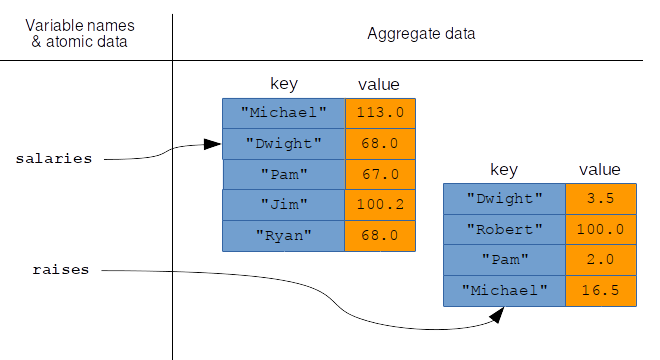
\includegraphics[width=0.9\textwidth]{vectorizedPandas.png}
\caption{Two \texttt{Series}es in memory}
\label{fig:vectorizedPandas}
\end{figure}

Consider the memory picture in Figure~\ref{fig:vectorizedPandas}. Here we have
two \texttt{Series}es, one pointed to by a \texttt{salaries} variable and the
other by \texttt{raises}, which are of different sizes and which have
overlapping, but not identical, sets of keys. What do you suppose Pandas would
do if we executed this code?

\begin{Verbatim}[fontsize=\small,samepage=true,frame=single,framesep=3mm]
new_salaries = salaries + raises
\end{Verbatim}

The answer, happily, is the smartest possible thing it could do. Pandas gets
neither confused nor stifled by the fact that the keys are in different orders
in the two \texttt{Series}es, and instead it does what you surely want:
add corresponding elements, with matching keys, and produce a new
\texttt{Series} with all of those sums.

\begin{figure}[ht]
\centering
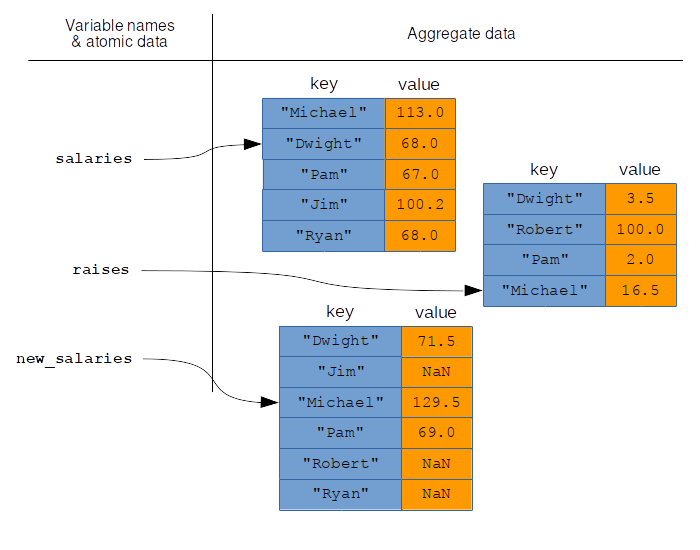
\includegraphics[width=0.8\textwidth]{vectorizedPandas2.png}
\caption{The result of \texttt{+}'ing two \texttt{Series}es that don't have all the same keys.}
\label{fig:vectorizedPandas2}
\end{figure}

The actual result in this case is in Figure~\ref{fig:vectorizedPandas2}, and
the output is here:

% salaries = pd.Series([113,68,67,100.2,68],
%   index=['Michael','Dwight','Pam','Jim','Ryan'])
% raises = pd.Series([3.5,100,2,16.5],
%   index=['Dwight','Robert','Pam','Michael'])

\begin{Verbatim}[fontsize=\small,samepage=true,frame=single,framesep=3mm]
new_salaries = salaries + raises
print(new_salaries)
\end{Verbatim}

\begin{Verbatim}[fontsize=\small,samepage=true,frame=leftline,framesep=5mm,framerule=1mm]
Dwight      71.5
Jim          NaN
Michael    129.5
Pam         69.0
Robert       NaN
Ryan         NaN
dtype: float64
\end{Verbatim}

\index{nan@\texttt{NaN} (``not a number'')}
\index{missing value}

Convince yourself that \texttt{Dwight}'s \$68,000 salary got added to his
\$3,500 raise, and that \texttt{Michael}'s \$113,000 was added to \$16,500,
\textit{etc.}

Don't get freaked out by those \texttt{NaN} entries just yet. The special value
``\textbf{NaN}'' stands for ``\textbf{not a number},'' and basically means that
Pandas has to throw up its hands in that case. And with good cause.
\texttt{Jim} has a current salary of \$100,200 in the first \texttt{Series},
but has no value at all in the second one (no raise for Jim this year? Haven't
decided what his raise will be yet? Something else?) and so Pandas shrugs and
says ``dunno.'' We say that the \texttt{Jim} entry in the
\texttt{new\_salaries} \texttt{Series} is a \textbf{missing value}. The same is
true for \texttt{Robert} and \texttt{Ryan}, each of whom was present in only
one of the two operands.

Now I know what you're thinking: ``can't Pandas just assume the salary and/or
raise is 0 if there's a missing one?'' The answer is that yes it can, but it
won't do so unless you give the go-ahead. Pandas is being cautious here, and
doesn't want to introduce errors into your data stream by false assumptions.
(Maybe in your company, for instance, there's a default entry-level salary that
every employee receives who's unspecified in the \texttt{salary}
\texttt{Series}. Or maybe the yearly raise is always assumed to be a flat 2.5\%
cost-of-living raise unless explicitly specified.)

\index{add@\texttt{add()} function (Pandas)}
\index{sub@\texttt{sub()} function (Pandas)}
\index{mul@\texttt{mul()} function (Pandas)}
\index{div@\texttt{div()} function (Pandas)}

If we do want Pandas to assume a certain default value, we have to change
tactics a bit and go with the \texttt{add()} function (or \texttt{sub()},
\texttt{mul()}, or \texttt{div()}):

\begin{Verbatim}[fontsize=\small,samepage=true,frame=single]
new_salaries = pd.Series.add(salaries, raises, fill_value=0)
print(new_salaries)
\end{Verbatim}

\begin{Verbatim}[fontsize=\small,samepage=true,frame=leftline,framesep=5mm,framerule=1mm]
Dwight      71.5
Jim        100.2
Michael    129.5
Pam         69.0
Robert     100.0
Ryan        68.0
dtype: float64
\end{Verbatim}

The \texttt{fill\_value} argument is the important one here: it specifies what
default value to use if one of the addends is missing a key from the other. Now
the result is as in Figure~\ref{fig:vectorizedPandas3}. You can, of course,
choose a \texttt{fill\_value} other than zero, if you wish.

\begin{figure}[ht]
\centering
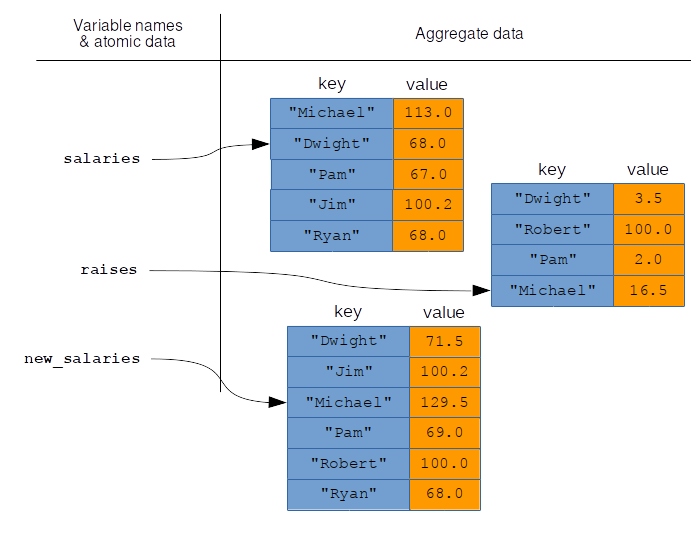
\includegraphics[width=0.8\textwidth]{vectorizedPandas3.png}
\caption{Using \texttt{add()} instead, and passing a \texttt{fill\_value}.}
\label{fig:vectorizedPandas3}
\end{figure}

As with NumPy arrays, we can add (or subtract, or multiply, ...) a single
atomic value to a series as well:

\begin{Verbatim}[fontsize=\small,samepage=true,frame=single,framesep=3mm]
cost_of_living_increase = salaries * .025
print(cost_of_living_increase)
\end{Verbatim}

\begin{Verbatim}[fontsize=\small,samepage=true,frame=leftline,framesep=5mm,framerule=1mm]
Michael    2.825
Dwight     1.700
Pam        1.675
Jim        2.505
Ryan       1.700
dtype: float64
\end{Verbatim}

\begin{Verbatim}[fontsize=\small,samepage=true,frame=single,framesep=3mm]
salaries = salaries + cost_of_living_increase
print(salaries)
\end{Verbatim}

\begin{Verbatim}[fontsize=\small,samepage=true,frame=leftline,framesep=5mm,framerule=1mm]
Michael    115.825
Dwight      69.700
Pam         68.675
Jim        102.705
Ryan        69.700
dtype: float64
\end{Verbatim}

It can sometimes be useful to do string concatenation as well, for instance if
we had employee first names and last names in two \texttt{Series}es with their
employee ID as the index:

\begin{Verbatim}[fontsize=\small,samepage=true,frame=single,framesep=3mm]
firsts = pd.Series(['Hannibal', 'Clarice', 'Multiple', 'Buffalo'],
    index=[666, 1993, 47, 988])
lasts = pd.Series(['Starling', 'Crawford', 'Lecter', 'Bill', 'Miggs'],
    index=[1993, 1650, 666, 988, 47])
print(firsts + " " + lasts)
\end{Verbatim}

\begin{Verbatim}[fontsize=\small,samepage=true,frame=leftline,framesep=5mm,framerule=1mm]
47        Multiple Miggs
666      Hannibal Lecter
988         Buffalo Bill
1650                 NaN
1993    Clarice Starling
dtype: object
\end{Verbatim}

\section{Copying \texttt{Series}es}

\section{Sorting \texttt{Series}es}
\index{in place}

\section{Concatenating and combining}

\section{Queries}

These functions are all summarized in Figure~\ref{fig:handySeries}.

\setlength\extrarowheight{5pt}

\begin{figure}[ht]
\centering
\begin{tabular}{c|p{3.3in}}
Function & Description \\
\hline

\texttt{len(}\textsl{arr}\texttt{)} & Get the number of elements in the array \textsl{arr}. \\

\textsl{arr}\texttt{[17]} & Get a specific element's value from the array \textsl{arr}. \\

\textsl{arr}\texttt{[8] =} (\textsl{something}) & Set a specific element of the array \textsl{arr}. \\

\textsl{arr} \texttt{+ 91} & Add a value to each element of \textsl{arr},
yielding a new array. (Also works with \texttt{-}, \texttt{*}, \texttt{/},
\textit{etc.}) \\

\textsl{arr1} \texttt{+} \textsl{arr2} & Add each pair of values in two arrays,
yielding a new array. (Also works with \texttt{-}, \texttt{*}, \texttt{/},
\textit{etc.}) \\

\textsl{arr1} = \textsl{arr2} & Make \textsl{arr1} point to the same data that
\textsl{arr2} points to. (\textit{Not} a copy!)\\

\textsl{arr1} = \textsl{arr2}\texttt{.copy()} & Make \textsl{arr1} point to a
new, independent copy of \textsl{arr2}. \\

\textsl{arr}\texttt{.sort()} & Sort the array \textsl{arr} \textbf{in place}. (Numerical or
alphabetical, depending on the \texttt{.dtype}.) \\

\texttt{np.sort(}\textsl{arr}) & Return a new array with the sorted elements
of \textsl{arr}. (Numerical or alphabetical, depending on the \texttt{.dtype}.)
\\

\texttt{np.append(}\textsl{arr}, \textsl{elem}\texttt{)} &
    Return a new array with \textsl{elem} tacked on to the end. \\

\texttt{np.append(}\textsl{arr1}, \textsl{arr2}\texttt{)} &
    Return a new array with the two arrays \textsl{arr1} and \textsl{arr2} concatenated. \\

\texttt{np.insert(}\textsl{arr}, \textsl{ind}, \textsl{val}\texttt{)} &
    Return a new array with the new value \textsl{val} inserted into position \textsl{ind} of \textsl{arr}. \\

\texttt{np.delete(}\textsl{arr}, \textsl{ind}\texttt{)} &
    Return a new array with the element at index \textsl{ind} removed from \textsl{arr}. \\

\texttt{np.flip(}\textsl{arr}\texttt{)} &
    Return a new array with \textsl{arr} in reverse order. \\
\end{tabular}
\bigskip
\caption{Handy functions, methods, and operators for Pandas \texttt{Series}es.}
\label{fig:handySeries}
\end{figure}
